\section{Web-Game [R]}
\setauthor{Rafetseder Tobias}
\subsection{Frontend [R]}
\subsubsection{Architektur [R]}
\subsubsection{p5.js [R]}
\subsection{Backend [R]}
\subsubsection{Node.js [R]}
\subsubsection{SocketIO [R]}
\subsection{Gamephysics [R]}
\subsection{Hitregistration [R]}
\subsection{Collisiondetection [R]}
\subsection{Regeln und Spielablauf [R]}
\section{Deployment [R]}
\setauthor{Rafetseder Tobias}
\subsection{Docker [R]}
\subsection{Leo-Cloud [R]}

% Ben dein teil kommt hier herein


\section{Map-Erkennung [H]}
\setauthor{Himmetsberger Jonas}
\subsection{Objekterkennung [H]}
\subsubsection{Beschreibung der Funktionalität [H]}
\subsection{Open-CV2 [H]}
\subsubsection{Umwandlung der Bilder in für das Spiel brauchbare Daten [H]}
\subsection{Kommunikation mit der Lobby via Flask und Flask SocketIO [H]}

\section{KI [H]}
\subsection{Lernen mit OpenAI-Gym [H]}
Der zweite Punkt ist die Künstliche Intelligenz. 
Im Laufe der Ausarbeitung der Diplomarbeit und der damit zusammenhängenden Forschung änderte sich oft die
Vorstellung darüber, wie das Endprodukt (KI) auszusehen hat, beziehungsweise, wie dieses aussehen kann. 
Limitierungen, welche vor der Forschung noch nicht bekannt und bewusst waren, begrenzten die Lernfähigkeit der KI.
Auf Probleme, Lösungen und Ergebnisse wird jedoch noch näher in ... eingegangen.
\subsection{Künstliche Intelligenz Definition [H]}
\subsection{Reinforcement Learning [H]}
\subsection{Die ScribbleFight-KI [H]}
\subsubsection{Beschreibung der Funktionalität [H]}
\subsubsection{Warum Python? [H]}
\subsection{Tensorflow und Keras [H]}
\subsubsection{Tensorflow [H]}
\subsubsection{Keras [H]}



% Siehe tolle Daten in Tab. \ref{tab:impl:data}.

% \begin{table}
%     \centering
%     \begin{tabular}{|lcc|}
%         \hline
%                   & \textbf{Regular Customers} & \textbf{Random Customers} \\ \hline
%         Age       & 20-40                      & \textgreater{}60          \\ \hline
%         Education & university                 & high school               \\ \hline
%     \end{tabular}
%     \caption{Ein paar tabellarische Daten}
%     \label{tab:impl:data}
% \end{table}

% \begin{figure}
%     \centering
%     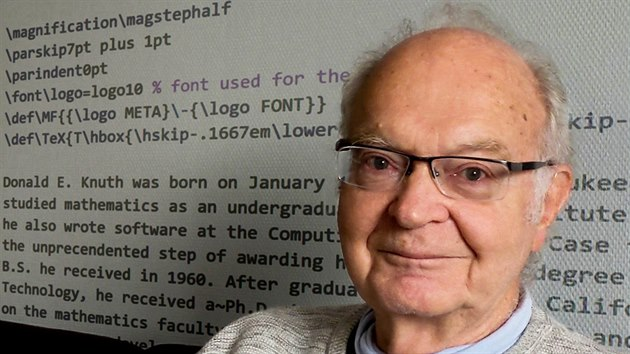
\includegraphics[scale=0.5]{pics/knuthi.jpg}
%     \caption{Don Knuth -- CS Allfather}
%     \label{fig:impl:knuth}
% \end{figure}

% Siehe und staune in Abb. \ref{fig:impl:knuth}.
% \lipsum[6-9]
% Dann betrachte den Code in Listing \ref{lst:impl:foo}.

% \begin{lstlisting}[language=Python,caption=Some code,label=lst:impl:foo]
% # Program to find the sum of all numbers stored in a list (the not-Pythonic-way)

% # List of numbers
% numbers = [6, 5, 3, 8, 4, 2, 5, 4, 11]

% # variable to store the sum
% sum = 0

% # iterate over the list
% for val in numbers:
%     sum = sum+val

% print("The sum is", sum)
% \end{lstlisting}